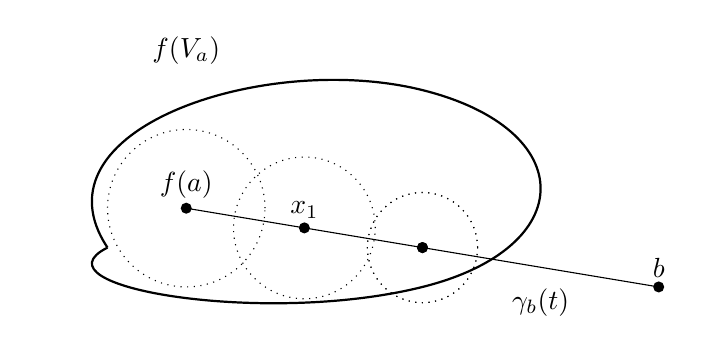
\begin{tikzpicture}[scale=1]
  \draw[thick] (-3,1.5) .. controls (-4,3) and (-1,4) .. (1,3.5)
    .. controls (3,3) and (3,1.5) .. (1,1)
    .. controls (-1,0.5) and (-4,1) .. (-3,1.5);
  \node at (-2,4) {$f(V_a)$};

  % Punto f(a)
  \fill (-2,2) circle (2pt);
  \node[above] at (-2,2) {$f(a)$};

  % Bola de radio r
  \draw[dotted] (-2,2) circle (1);

  % Punto f(a2)
  \fill (-0.5,1.75) circle (2pt);
  \node[above] at (-0.5,1.75) {$x_1$};

  % Bola de radio r
  \draw[dotted] (-0.5,1.75) circle (0.9);

  % Punto f(a3)
  \fill (1,1.5) circle (2pt);

  % Bola de radio r
  \draw[dotted] (1,1.5) circle (0.7);

  % Punto f(a3)
  \fill (1,1.5) circle (2pt);

  % Bola de radio r
  \draw[dotted] (1,1.5) circle (0.7);

  % Punto b
  \fill (4,1) circle (2pt);
  \node[above] at (4,1) {$b$};

  % Recta
  \draw (-2,2) -- (4,1);
  \node[above] at (2.5,0.5) {$\gamma_b(t)$};
\end{tikzpicture}
